\subsection{Modelo Fisico}
\subsubsection{Motor elegido}
El motor elegido para implementar la solucion es \textbf{Microsoft Sql Server 2008} junto a sus herramientas graficas.

\subsubsection{Diagrama fisico}
\begin{landscape}
	\begin{figure}[t]
	  \centering
		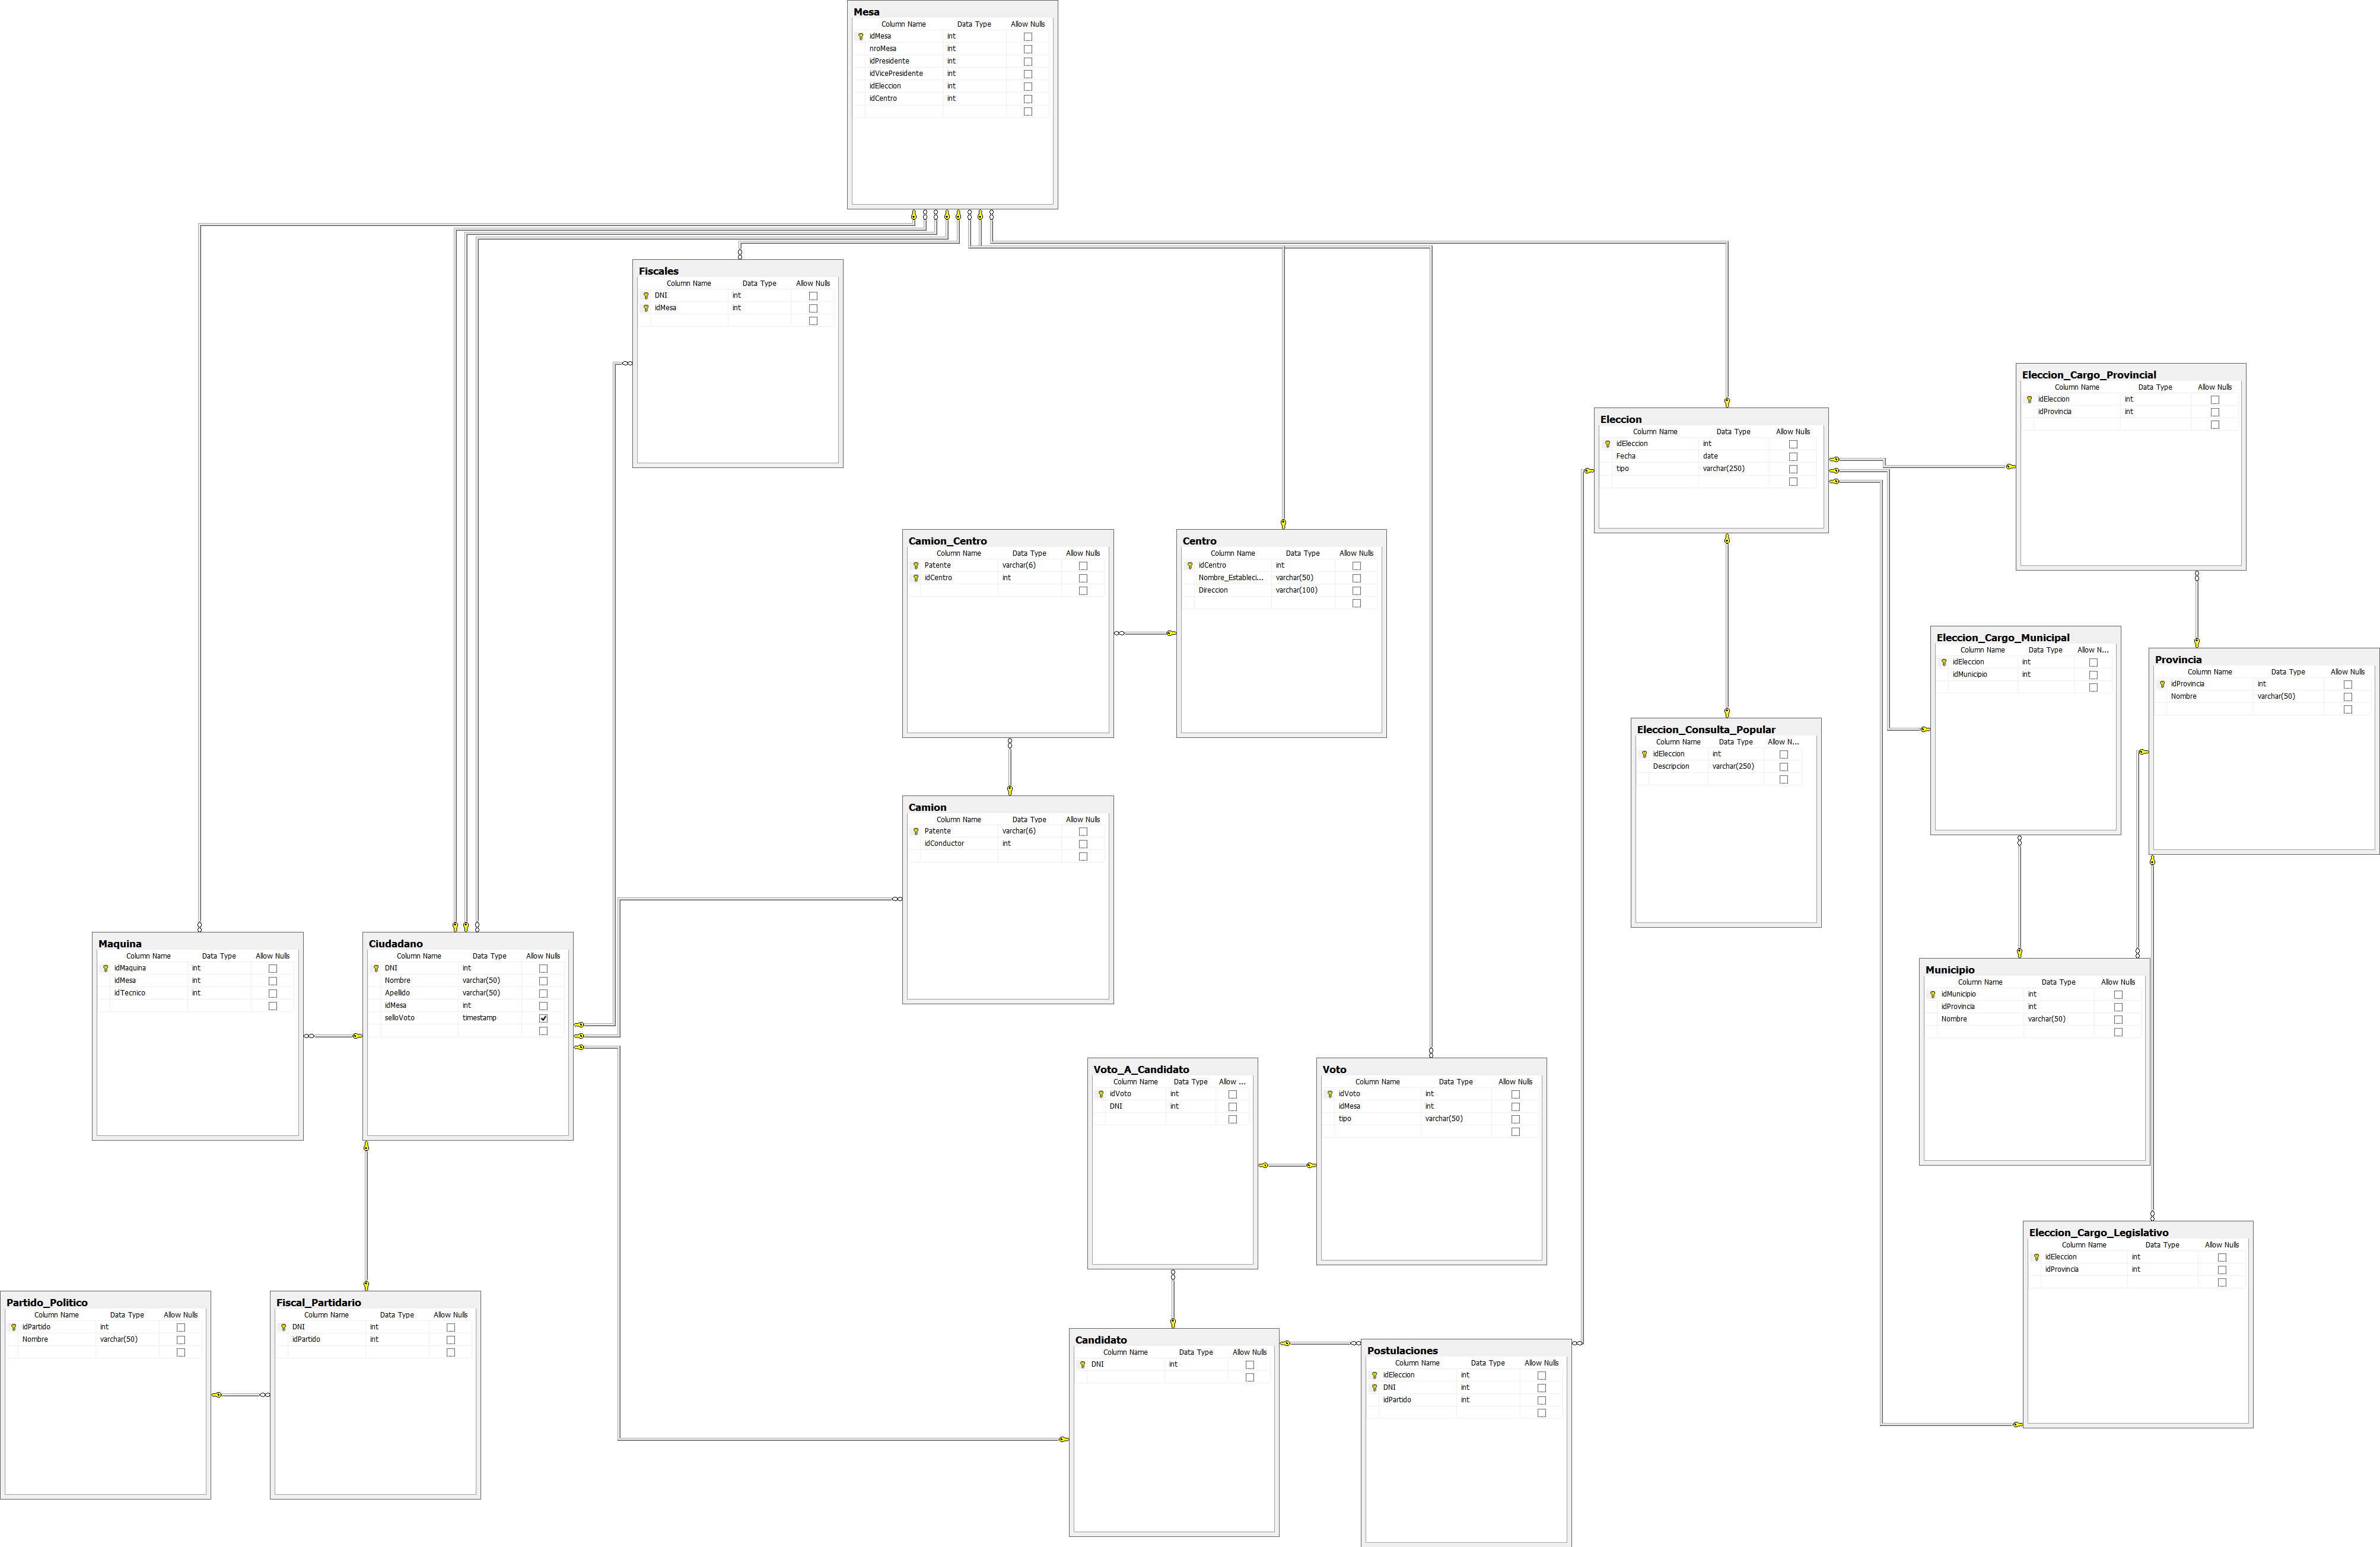
\includegraphics[scale=0.35]{fig/modelo-fisico.png}
	  \caption{Diagrama fisico.}
	\end{figure}
\end{landscape}

\subsubsection{Modelado fisico de las restricciones con triggers}
Modelaremos las restricciones al modelo utilizando funcionalidades provistas por el motor de la base de datos, como ser \textbf{Stored Procedures}, \textbf{Triggers}, \textbf{Checks}, etc. segun nos parezca conveniente. A continuacion se presenta el modelado de las restricciones. La notacion utilizada es: Restricciones resueltas, soluciones itemizadas de forma anidada. 

\begin{itemize}
%------------------------- Done -------------------------
		\item[$\bigstar$] Los campos tipo de las tablas con jerarquia disjunta deben contener los valores correctos. 
		\begin{itemize}
			\item[\Checkmark] Se crearon \textbf{Check Constraints} para validar los campos \texttt{tipo} de las tablas que tienen jerarquias disjuntas.
		\end{itemize}
\end{itemize}
\vspace{1.2cm}
\begin{itemize}
%------------------------- Done -------------------------
		\item[$\bigstar$] Todos los votos para una eleccion son: o bien consulta popular o bien de tipo candidato según corresponda el tipo de eleccion.
		\item[$\bigstar$] Si la eleccion es una consulta popular, los votos deben ser si/no. Sino, deben ser candidatos.
		\begin{itemize}
			\item[\Checkmark] \textbf{After Insert trigger} sobre tabla voto. navegamos a mesa y de mesa a eleccion y chequeamos que el campo tipo de la eleccion corresponda con el campo tipo del voto. Sino, rollbackeamos.
		\end{itemize}
\end{itemize}
\vspace{1.2cm}
\begin{itemize}
%------------------------- Done -------------------------
		\item[$\bigstar$] Un voto a candidato, debe referenciar a un candidato postulado para dicha eleccion.
		\begin{itemize}
			\item[\Checkmark] \textbf{After Insert trigger} sobre tabla voto a candidato. Navegamos a Voto, luego a Mesa y obtenemos el idEleccion. Luego buscamos los postulados a dicha eleccion y verificamos que el voto sea valido. Sino, rollbackeamos.
		\end{itemize}
\end{itemize}
\vspace{1.2cm}
\begin{itemize}
%------------------------- Done -------------------------
		\item[$\bigstar$] No hay candidatos repetidos en una eleccion.
		\begin{itemize}
			\item[\Checkmark] Queda determinado por la \textbf{PK} de la tabla Postulaciones.
		\end{itemize}
\end{itemize}
\vspace{1.2cm}
\begin{itemize}
%------------------------- Done -------------------------
		\item[$\bigstar$] Cada partido politico presenta un solo candidato por eleccion.
		\begin{itemize}
			\item[\Checkmark] \textbf{Check Constraint Unique} (idEleccion, idPartidoPolitico) en postulaciones.
		\end{itemize}
\end{itemize}
\vspace{1.2cm}
\begin{itemize}
%------------------------- Done -------------------------	
		\item[$\bigstar$] La suma de los votos de todas las mesas de todos los candidatos debe ser menor o igual(votos en blanco diferencia) a la cantidad de ciudadanos que tiene el datetime cuandoVoto? No nulo en el padron de dicha eleccion. (notar que esto tambien lo acota por la cantidad de ciudadanos). 
		\item[$\bigstar$] \fk{Alguien piense esto a ver si no estoy flasheando plz.}
		\begin{itemize}
			\item{Queda implicada por el stored procedure de voto, que chequea sello null y marca no null el sello luego. No hay forma que de se inserten mas votos que personas}.
		\end{itemize}
\end{itemize}
\vspace{1.2cm}
\begin{itemize}
%------------------------- Done -------------------------
		\item[$\bigstar$] Un ciudadano vota en una sola mesa por eleccion.
		\begin{itemize}
			\item[\Checkmark] \textbf{Instead of Insert trigger} en Padron que verifique que para ese DNI, no exista otra mesa, de la misma eleccion, que ya lo tenga asociado. Si no existe la relacion entre dni, mesa y eleccion, se inserta el registro correspondiente.
		\end{itemize}
\end{itemize}
\vspace{1.2cm}
\begin{itemize}
%------------------------- Done -------------------------
		\item[$\bigstar$] Una maquina funciona en una sola mesa por eleccion.
		\begin{itemize}
			\item[\Checkmark] \textbf{Instead of Insert Trigger} en Mesa para ver que la maquina asignada no este asignada a otra mesa en esa eleccion. Si no existe una mesa de esta eleccion con esa maquina, se inserta la relacion. 
		\end{itemize}
\end{itemize}
\vspace{1.2cm}
\begin{itemize}
%------------------------- Pending -------------------------
		\item[$\bigstar$] Un ciudadano no pueda ser mas que una y solo una de estas opciones: conductor, tecnico, presidente, vicepresidente, candidato o fiscal en una misma eleccion.
		\begin{itemize}
			\item[\Checkmark] \textbf{Constraint Check}: las FK de presidente y vicepresidente deben referenciar distintos ciudadanos por mesa.
			
			\item[\Checkmark] \textbf{Instead of Insert trigger} en Mesa que verifique que las personas referenciadas por idPresidente y idVicepresidente no participan en ningun otro cargo (conductor, tecnico, candidato o fiscal) en esa eleccion.
			
			\item[\Checkmark] \textbf{Instead of Insert trigger} en Camion que verifique que la persona referenciada por idConductor no participa en ningun otro cargo (presidente, vicepresidente, tecnico, candidato o fiscal) en esa eleccion.

			\item[\Checkmark] \textbf{Instead of Insert trigger} en Maquina que verifique que la persona referenciada por idTecnico no participa en ningun otro cargo (presidente, vicepresidente, conductor, candidato o fiscal) en esa eleccion.

			\item[\Checkmark] \textbf{Instead of Insert trigger} en Postulaciones que verifique que la persona referenciada por DNI no participa en ningun otro cargo (presidente, vicepresidente, conductor, tecnico o fiscal) en esa eleccion.

			\item[\Checkmark] \textbf{Instead of Insert trigger} en Fiscales que verifique que la persona referenciada por DNI no participa en ningun otro cargo (presidente, vicepresidente, conductor, tecnico o candidato) en esa eleccion.
		\end{itemize}	
\end{itemize}
\vspace{1.2cm}
\begin{itemize}
%------------------------- Falta codearlos bien -------------------------
		\item[$\bigstar$] Toda persona que vota en una mesa, debe tener nulo el campo selloVoto del padron para dicha mesa. ie. No permitir que la gente vote mas de una vez por eleccion.
		\item[$\bigstar$] Para todo voto que se inserta se debe actualizar correctamente la fecha y hora en la que voto y poniendo el “sello” virtual en el padron asignando un valor no nulo a cuandoVoto.
		\item[$\bigstar$] Para todo voto que se inserta se debe actualizar correctamente la tabla hija de ser necesario. ie Voto y Voto A Candidato.
		\item[$\bigstar$] Validar que el voto puede hacerse en la fecha de la eleccion de 8am a 6pm.
		\begin{itemize}
			\item[\Checkmark] Con respecto a las restricciones referidas al voto y el sello en el padron, no podemos modelarlas con before y after triggers dado que no tenemos forma de navegar desde la tabla voto hacia el padron(no se guarda info de la persona en la tabla voto.). Con lo cual crearemos un stored procedure, que realizará la operacion de voto como una transacción, verificando que el sello sea NULO antes de insertar el voto y que el sello contenga el datetime una vez insertado el voto. Ademas de realizar la consistencia de insercion del voto si es a candidato en varias tablas. Las validaciones adicionales al voto mencionadas anteriormente, estan contempladas dentro de este procedimiento pues las tablas involucradas ya contienen los triggers necesarios.
		\end{itemize}
\end{itemize}
\vspace{1.2cm}
\begin{itemize}
%------------------------- Pending -------------------------
	\item[$\bigstar$] Inserciones consistentes en tablas con jerarquia: ie. Entidades: Ciudadano, Eleccion, Voto y sus hijos. 
	\begin{itemize}
		\item[\Checkmark] Dado que la PK de la tabla hijo es FK de la PK de la tabla padre, la insercion en tablas hijos fallara si no existe el registro correspondiente en la tabla padre. Analogamente, debemos proveer mecanismos para poder realizar inserciones consistentes de entidades padres que requieran insercion en tablas hijas. Para la tabla Voto, el punto anterior resuelve esto. Ciudadano no tiene herencia disjunta, con lo cual, no es necesario proveer este mecanismo. Se proveera un mecanismo (\textbf{Stored Procedure}) para crear elecciones de diferentes tipos. 
	\end{itemize}
\end{itemize}


\fk{OJO QUE VAMOS A TENER QUE USAR TRANSACCIONES EN LOS STORED PROCEDURES.}
ojo con los \textbf{insert triggers} y los updates, habria que prohibir los updates o hacer triggers en insert y update?
no se deberian permitir deletes ni updates sobre voto(y posiblemente otras tablas). ??

\subsubsection{Stored Procedures}
Estos procedimientos permiten realizar operaciones que involucran mas de una operacion en la base de datos de manera atomica.
\begin{itemize}
	\item Voto a candidato(dniVotante, dniCandidato, idMesa)
	\item Voto a consulta popular(dniVotante, idMesa, respuestaPlesbicito)
	\item Crear eleccion(tipo)
\end{itemize}